\section{Numerical evidence and a sharpened conjecture}
\label{sec:evidence}

The results above prove the conjecture of Ref.~\cite{namba2026arrow} for Gaussian states and reduce it, for general states of the pendulum, mainly to a bound on the focus slope. Here we summarize the numerical evidence for the general case. All evaluations are exact up to quadrature error: the posterior moments of Gaussian mixtures are evaluated in closed form, the remaining integrals on adaptive or nested grids, and every reported number was checked against at least one refined grid (Appendix~\ref{app:methods}).

\emph{Searches.} For the pendulum we evaluated random Gaussian mixtures with $K = 2$ to $40$ components, families that vary one parameter at a time, and adversarial searches that maximize $R$, the covariance term, the mass of valleys, the fraction $(R - L)/(\kappa - L)$ of the available room that a state uses, and the advantage $g^*$. Together with the quartic oscillator, the double well and the twist flow, more than $2{,}300$ distinct states were stored and re-evaluated. No state had $R > \kappa$.

\emph{Near the hyperbolic point.} Let $\kappa - L$ be the distance of the law term from $\kappa$. Among states with small distance, the largest excess $R - L$ found decreases at least linearly with the distance: the upper envelope has slope $0.98$ between distances $3\times10^{-4}$ and $3\times10^{-3}$, and $1.26$ over the whole range, and states closer than $3\times10^{-3}$ use at most $9\%$ of the available room. The variance of the local strain $\bar a$ decreases as the square of the distance, because the strain is flat at its maximum, while the focus mismatch $\E\|H - F\|/\tr F$ stays of order one.

\emph{States that use almost all of the room.} The fraction of room used can be pushed towards $1$, but only from below and only through a ruler effect: a needle at $q = \pi$ that carries a small part of the weight but almost all of the Fisher information sets $R$, while a broad component far from the maximum enlarges the distance $\kappa - L$. Along a sequence of shrinking needles we observed that $R$ stays below the critical rate of the needle alone, which is below its strain and below $1$ by Theorem~\ref{thm:gaussian}.

\emph{Gap.} For $\sigma \leq 10^{-2}$ every stored pendulum state has $(1-R)/\sigma \geq 0.946$; the smallest values belong to the fans of Sec.~\ref{sec:mixtures}, whose advantage over the best Gaussian state saturates at about $5\%$ of the Gaussian gap. In the other flows the gap is also proportional to $\sigma$ (Fig.~\ref{fig:flows}).

\begin{figure*}[t]
\centering
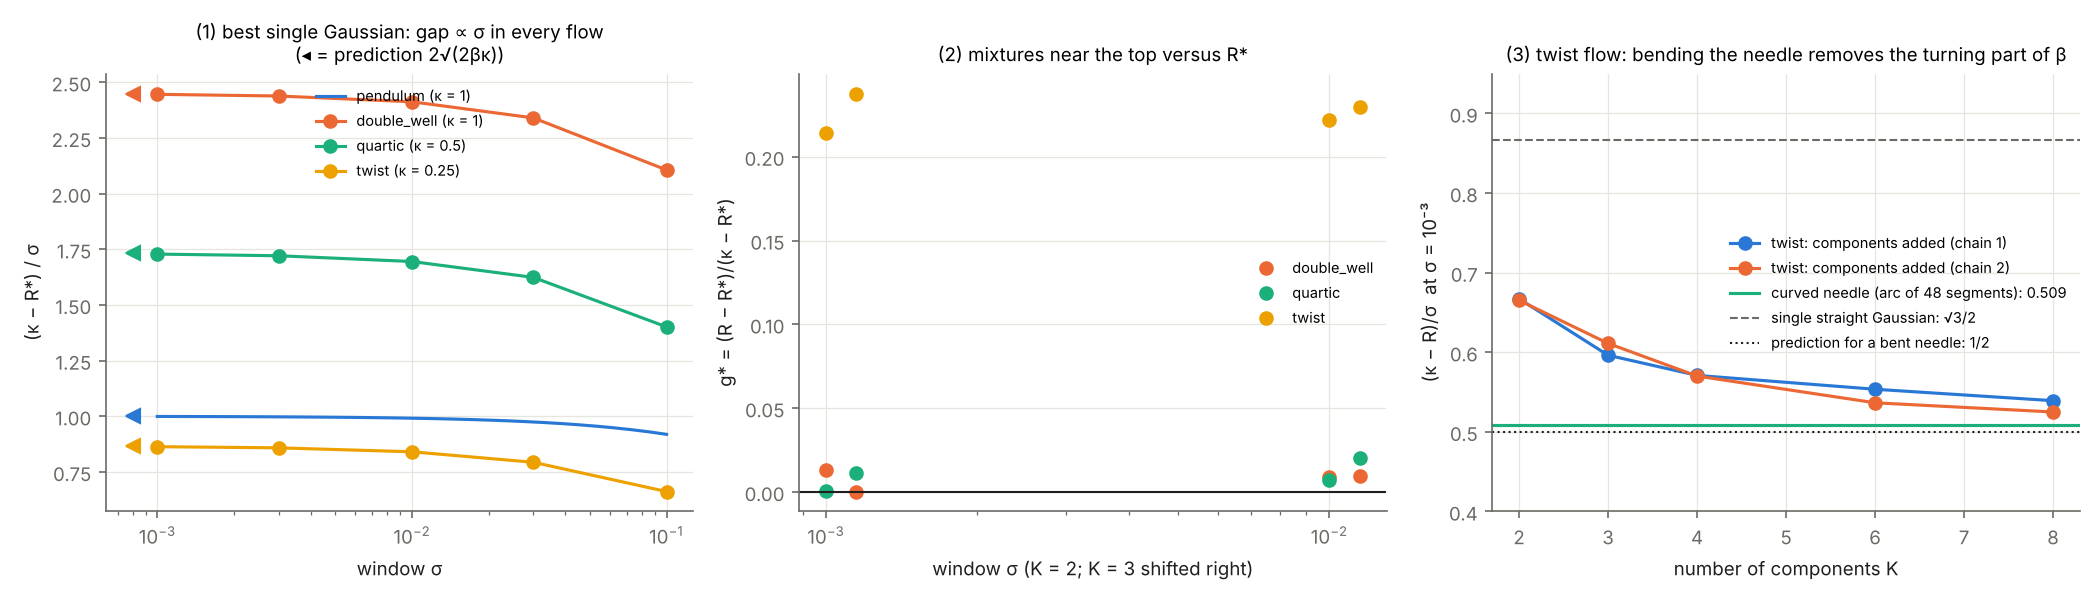
\includegraphics[width=0.95\textwidth]{figures/fig4_flows.png}
\caption{Resolution gap in four flows. (1) Best Gaussian state: $(\kappa - R^*)/\sigma$ against $\sigma$; triangles mark the prediction $2\sqrt{2\beta\kappa}$ of Proposition~\ref{prop:gap}. (2) Advantage $g^*$ of mixtures near the maximal strain. (3) Twist flow: gap of mixtures with $K$ components, of a bent needle, of the best straight Gaussian state ($\sqrt3/2$) and the prediction $1/2$ for a needle that follows the rotation.}
\label{fig:flows}
\end{figure*}

These observations suggest a sharpened form of the conjecture.

\begin{gapconjecture}
For the pendulum there are constants $c > 0$ and $\sigma_0 > 0$ such that every state satisfies $\kappa - R \geq c\,\sigma$ for $\sigma \leq \sigma_0$. Numerically, the best constant is close to $0.95$.
\end{gapconjecture}

The resolution-gap conjecture implies Conjecture~1 of Ref.~\cite{namba2026arrow} for the pendulum at small resolution, with a margin. By Theorem~\ref{thm:statewise} it would follow from a lower bound on $\Theta'$ that holds uniformly over states, together with $\tilde\varepsilon + D = o(\sigma)$. We expect the same structure, a gap $c_f\,\sigma$ with $c_f$ set by the curvature of the strain at its maximum after any rotation of the stretching direction has been followed, for other Hamiltonian flows with finite $\kappa$.
